\section{Durchführung}
\label{sec:Durchführung}

\subsection{Versuchsaufbau}
\label{sec:Versuchsaufbau}
%\begin{figure}
%	\centering
%	\caption{Schematische Darstellung des Versuchsaufbaus \cite{anleitung}.}
%	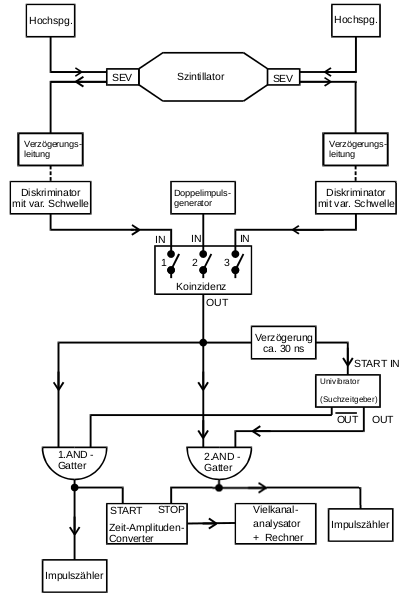
\includegraphics{Bilder/aufbau.png}
%	\label{fig:aufbau}
%\end{figure}
%
%\begin{figure}
%	\centering
%	\caption{Schematische Darstellung der Quelle zur Erzeugung radioaktiven Isotopen \cite{anleitung}.}
%	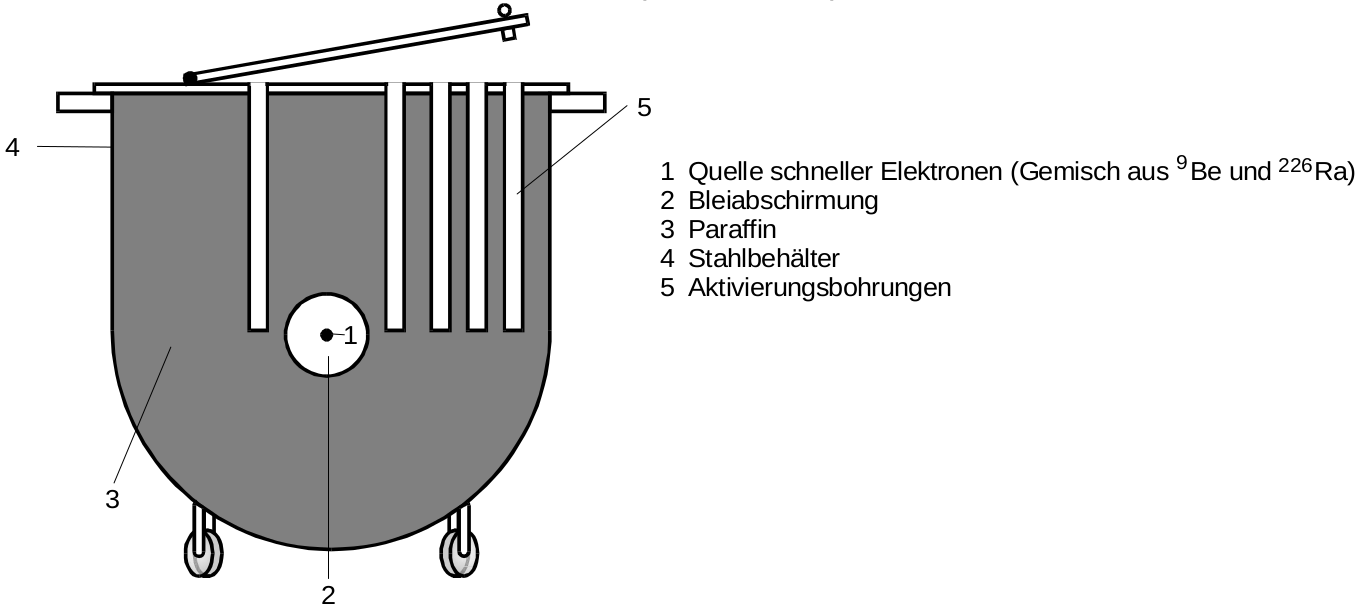
\includegraphics{content/toepfchen.png}
%	\label{fig:kochen}
%\end{figure}
%
Der Versuchsaufbau -- wie in Abbildung \ref{fig:aufbau} dargestellt -- besteht im Wesentlichen 
aus einem zerfallenden radioaktiven Isotop und einem Geiger-Müller-Zählrohr, welches die 
zerfallenden Kerne misst.
Das Geiger-Müller-Zählrohr ist entspricht einer mit Gas gefüllten Röhre. Trifft ein $\beta$-
oder $\gamma$- Teilchen auf ein Gasteilchen wird dieses ionisiert und kann aufgrund einer
anliegenden Spannung an der Röhre gemessen werden.
Dabei werden die gemessenen Zerfälle pro Messzeitintervall, welches am Zeitgeber einstellbar 
ist, an den Zählern 1 und 2 angezeigt. Nach jedem Messvorgang wird der Zähler umgeschaltet und 
der vorherige Wert auf dem aktuellen Zähler wird überschrieben. Der Versuchsaufbau ist mit
einer Blei-Abschirmung ausgestattet um die radioaktive Strahlung abzuschirmen.

Zur Erzeugung der radioaktiven Isotope wird das Objekt in Abbildung \ref{fig:kochen} verwendet.
Hierbei werden stabile Kerne mit niederenergetischen Neutronen beschossen. 
Da die Neutronen ihre Energie durch elastische Stöße an die Kerne übergeben und die maximale
Energie bei gleichen Massen der Stoßpartner erreicht wird, werden die Neutronen in einem 
Paraffinmantel gebremst, bis sie die optimale Energie besitzen.


\subsection{Versuchsbeschreibung}
\subsubsection{für die Ablenkung im elektrischen Feld}
In der ersten Messung soll die Proportionalität zwischen der Leuchtfleckverschiebung $D$ und der 
Ablenkspannung $U_{\mathrm{d}}$ überprüft werden. Diese Messung wird für drei verschiedene 
Beschleunigungsspannungen $U_{\mathrm{B}}$ durchgeführt.
Bevor die Spannungsversorgung der Kathodenstrahlröhre angeschaltet wird, muss der Schalter 
circa eine Minute als Anheizzeit in der Stellung "STANDBY" stehen. Wenn der Leuchtfleck
zu unscharf wird, kann dieser durch Regulierung der Fokussierungs- und 
Wehnelt-Spannung fokussiert werden.
Das Koordinatennetz, auf dem die Verschiebung des Leuchtflecks abgelesen wird, hat neun 
äquidistante (Abstand: $1 inch$) Linien. Der Leuchtfleck soll bei Variation der 
Ablenkspannung $U_{\mathrm{d}}$ auf die neun Linien positioniert werden. Ist dies der Fall,
wird jeweils die Verschiebung als $n*1inch$ und die zugehörige Ablenkspannung 
$U_{\mathrm{d}}$ abgelesen. Es ergeben sich also neun Messtupel.

Für die Bestimmung einer unbekannten Frequenz einer Sinusspannung wird der 
Kathodenstrahl-Oszillosgraph verwendet. Es wird Sägezahnfrequenz solange variiert bis 
stehende Wellen zu erkennen sind. Dann wird die zugehörige Frequenz notiert. 
Es sollen vier Frequenzen für die Verhältnisse $n = \frac{1}{2}, 1, 2$ und $3$ bestimmt werden.
Damit der Leuchtschirm nicht beschädigt wird, sollte der Elektronenstrahl nicht zu lange auf 
die gleiche Stelle abgelenkt werden.

\subsubsection{für die Ablenkung im magnetischen Feld}
Die Leuchtfleckverschiebung $D$ in Abhängigkeit von der Flussdichte $B$ wird für die 
Beschleunigungsspannungen $U_{\mathrm{B}}=\SI{250}{\volt}$ und $U_{\mathrm{B}}=\SI{450}{\volt}$
gemessen. Damit nur das Magnetfeld des Spulenpaares auf die Kathodenstrahlöhre wirkt
wird die Kathodenstrahlöhre in Richtung der Horizontalkomponente des Erdmagnetfeldes verschoben.
Diese Richtung kann mit dem Deklinatorium-Inklinatorium bestimmt werden, indem dieser einen 
Winkel von $0°$ anzeigt. Der Strom soll wieder abgelesen werden, wenn sich der 
Leuchtfleck auf den äquidistanten Linien befindet.

Für die Bestimmung der Horizontalkomponente des Erdmagnetfeldes $B_{\mathrm{hor}}$ wird eine 
möglichst niedrige Beschleunigungsspannung verwendet. 
Der Spulenstrom wird ausgeschaltet und die Kathodenstrahlröhre wieder in die Richtung der 
Horizontalkomponente des Erdmagnetfeldes gedreht. Die Position des abgelenkten Leuchtflecks 
auf dem Schirm wird markiert. Daraufhin wird die Kathodenstrahlröhre um $90°$ gedreht und 
der Spulenstrom wieder hochgeregelt bis das Erdmagnetfeld wieder auf die vorherige Ablenkung
kompensiert wird. Der kompensierende Spulenstrom wird notiert.
